\chapter{Recalculation}
\label{ch:recalc}

\section{When it happens}
\index{recalculation}

After every change to every cell --- unless you have turned that off.

A workbook with no formulas in it skips the whole business, which is why typing
into a plain table of numbers is instant and typing into a worksheet full of
totals is not.

\section{How it happens}
\index{recalculation!method}

\ccprod{} keeps no record of which formula depends on which cell. Building and
maintaining a dependency graph would cost memory the machine does not have, so
instead the order of evaluation is \emph{discovered}, by repeated passes.

\begin{ccprocedure}[What a recalculation does]
\item Every formula in every worksheet is marked out of date.
\item A pass sweeps them all. A formula whose inputs are all up to date is
evaluated and marked done. A formula that reads something still out of date is
left alone and its provisional answer thrown away.
\item Step 2 repeats until nothing is out of date --- or until a pass changes
nothing at all.
\item Anything still out of date after a pass that achieved nothing is marked
\errv{\#CYCLE!}.
\end{ccprocedure}

\begin{ccfigure}
\begin{tikzpicture}[x=1pt,y=-1pt,
   cel/.style={draw=ccink,line width=0.6pt,minimum width=44pt,
               minimum height=15pt,inner sep=1pt,
               font=\ttfamily\fontsize{7.6}{9}\selectfont},
   done/.style={cel,fill=black!12},
   lab/.style={font=\sffamily\bfseries\fontsize{7.6}{9}\selectfont,
               text=ccink,anchor=east},
   note/.style={font=\sffamily\fontsize{7.2}{8.8}\selectfont,text=ccink,
                anchor=west}]

  \foreach \p/\y in {1/0,2/30,3/60}{
    \node[lab] at (-6,{\y+8}) {Pass \p};
  }

  % pass 1
  \node[cel]  at (22,8)  {A1 =B1+1};
  \node[cel]  at (74,8)  {B1 =C1*2};
  \node[done] at (126,8) {C1 =5};
  \node[note] at (156,8) {C1 is a constant, so B1 can go next time};

  % pass 2
  \node[cel]  at (22,38)  {A1 =B1+1};
  \node[done] at (74,38)  {B1 = 10};
  \node[done] at (126,38) {C1 =5};
  \node[note] at (156,38) {B1 settles at 10};

  % pass 3
  \node[done] at (22,68)  {A1 = 11};
  \node[done] at (74,68)  {B1 = 10};
  \node[done] at (126,68) {C1 =5};
  \node[note] at (156,68) {A1 settles. Nothing left out of date; stop};

  \node[font=\sffamily\fontsize{7.2}{8.8}\selectfont,text=ccink,anchor=west]
    at (-6,92) {Shaded cells are up to date at the end of that pass.};
\end{tikzpicture}
\caption{A three-deep chain settling in three passes}
\label{fig:recalcpasses}
\end{ccfigure}

Two useful things fall out of this.

\begin{ccsteps}
\item \textbf{The order you typed the formulas in does not matter.} A formula
written before the cell it depends on resolves perfectly well; it just takes
one more pass.
\item \textbf{Circular references are detected for free.} A pass that makes no
progress means the remaining formulas can only be waiting on each other, which
is the definition of a cycle. There is no separate check.
\end{ccsteps}

The cost is speed: a chain ten formulas deep takes ten passes over the whole
workbook. Deep chains of single-cell dependencies are the slowest thing you can
build. A worksheet of a hundred formulas that all read constants recalculates in
one pass; a worksheet of a hundred formulas in one long chain takes a hundred.

\section{Turning it off}
\index{recalculation!manual}\index{Auto recalc command}\index{Recalc now command}

On a worksheet with a long chain of formulas, recalculating after every
keystroke-and-\key{Return} is the slowest part of typing. Two commands exist for
that.

\begin{cctable}{Command}{Effect}{2.2in}{2.62in}
\menupath{Data > Auto recalc} & Turns automatic recalculation off, or back on.
One command for both: it is a switch. \\
\menupath{Data > Recalc now} & Recalculates immediately, whether the switch is
on or off. \\
\end{cctable}

Neither has a keyboard shortcut. \ccprod{} starts with automatic recalculation
on.

\subsection{Knowing which mode you are in}

With the switch off, the right-hand end of the status line says so:

\begin{ccfigure}
\ccscreenscale{1.4}
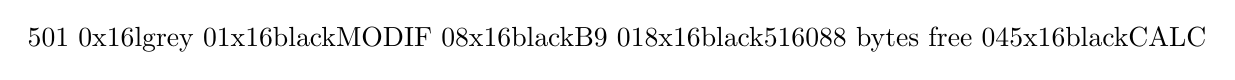
\begin{tikzpicture}
\node[inner sep=0pt,anchor=north west] (rc) at (0,0) {%
\ccscreenbegin{50}{1}
  \ccfillrow{0}{x16lgrey}
  \cctext{0}{1}{x16black}{MODIF}
  \cctext{0}{8}{x16black}{B9}
  \cctext{0}{18}{x16black}{516088~bytes~free}
  \cctext{0}{45}{x16black}{CALC}
\ccscreenend
};
\end{tikzpicture}
\caption{Manual recalculation, with an answer on screen that is out of date}
\label{fig:recalcind}
\end{ccfigure}

\begin{cctable}{Indicator}{Means}{0.85in}{3.97in}
\msg{CALC} & The switch is off \emph{and} something has changed. \textbf{The
answers on screen are stale.} \\
Nothing & Everything else: either automatic recalculation is on, or it is off
and nothing has changed since the last one. Either way the screen is
current. \\
\end{cctable}

\begin{ccnote}
There is no indicator for ``switched off, and up to date''. \ccprod{} used to
show \msg{MANUAL} for that and the word was dropped: it is not a state worth a
permanent warning, and it turns into \msg{CALC} on the very next edit anyway.
\end{ccnote}

\begin{cccaution}
\msg{CALC} means the numbers you are looking at are wrong. They are the answers
to the question the worksheet used to ask.

Press \menupath{Data > Recalc now} before reading anything off a worksheet
showing \msg{CALC}, and before saving one --- a workbook saved in that state
stores the stale values, and opening it again will not recalculate them until
something is changed.
\end{cccaution}

\subsection{Switching back on}

Turning automatic recalculation back on recalculates at once if anything was
skipped while it was off. The point of the switch is to defer the work, not to
lose it.

Turning it \emph{off} does nothing immediately; it just stops.

\section{Everything is recalculated}

The sweep covers every worksheet in the workbook, not just the one on screen.
That is what makes a chain running from \emph{Q1} through \emph{Q2} to
\emph{Summary} settle correctly no matter which sheet you are editing.

\section{Circular references}
\index{circular reference}\index{CYCLE error}

A formula that depends on itself, directly or through others, displays
\errv{\#CYCLE!}.

\begin{ccexamples}[]{0.44\linewidth}
\exn{A1: =A1+1}{\#CYCLE!}{direct}
\exn{A1: =A2 / A2: =A1}{\#CYCLE!}{indirect}
\exn{A6: =SUM(A1:A6)}{\#CYCLE!}{the range covers its own cell}
\end{ccexamples}

Every cell in the cycle is marked, and so is every cell that depends on one.
Cells that have nothing to do with the cycle are unaffected and keep their
correct values.

\begin{ccnote}
\ccprod{} shows \errv{\#CYCLE!} in the cell. Excel shows 0 and a warning in its
status bar; Lotus~1-2-3 showed a \msg{CIRC} indicator. \ccprod's answer is the
most direct of the three: the cell that is wrong is the cell that says so.
\end{ccnote}

There is no iterative calculation. A cycle is always an error, and there is no
setting that makes \ccprod{} converge on one instead.

\section{Formulas that never recalculate}

Two kinds of cell look like formulas and do not behave like them.

\begin{ccsteps}
\item \textbf{Formulas imported from an \fname{.XLSX} that \ccprod{} could not
compile.} They hold the value Excel last calculated. They are not formulas any
more, and they will not change. See Chapter~\ref{ch:importexport}.
\item \textbf{Formulas the program cannot reach.} If one of the program's files
is missing from the card, recalculation cannot run at all and every formula
keeps its previous value, silently. See Chapter~\ref{ch:installing}.
\end{ccsteps}

In both cases the formula bar is the way to tell: a cell that is still a formula
shows its formula there.
